\documentclass[11pt]{article}

\usepackage{graphicx}
\usepackage{fullpage}
\usepackage{mathptmx}
\usepackage[T1]{fontenc}
\usepackage{hyperref,microtype,pdfsync}
\usepackage{amsmath,amsfonts,amssymb,amsthm}
\usepackage{mathtools}
\usepackage{fancyhdr}

%%% BLACKBOARD SYMBOLS

% hyperref package defines C and G, undefined to avoid conflicts
\let\C\relax
\let\G\relax
\newcommand{\C}{\ensuremath{\mathbb{C}}}
\newcommand{\D}{\ensuremath{\mathbb{D}}}
\newcommand{\F}{\ensuremath{\mathbb{F}}}
\newcommand{\G}{\ensuremath{\mathbb{G}}}
\newcommand{\J}{\ensuremath{\mathbb{J}}}
\newcommand{\N}{\ensuremath{\mathbb{N}}}
\newcommand{\Q}{\ensuremath{\mathbb{Q}}}
\newcommand{\R}{\ensuremath{\mathbb{R}}}
\newcommand{\T}{\ensuremath{\mathbb{T}}}
\newcommand{\Z}{\ensuremath{\mathbb{Z}}}
\newcommand{\QR}{\ensuremath{\mathbb{QR}}}

\newcommand{\Zt}{\ensuremath{\Z_t}}
\newcommand{\Zp}{\ensuremath{\Z_p}}
\newcommand{\Zq}{\ensuremath{\Z_q}}
\newcommand{\ZN}{\ensuremath{\Z_N}}
\newcommand{\Zps}{\ensuremath{\Z_p^*}}
\newcommand{\ZNs}{\ensuremath{\Z_N^*}}
\newcommand{\JN}{\ensuremath{\J_N}}
\newcommand{\QRN}{\ensuremath{\QR_{N}}}
\newcommand{\QRp}{\ensuremath{\QR_{p}}}

%%% THEOREM COMMANDS

\theoremstyle{plain}            % following are "theorem" style
\newtheorem{theorem}{Theorem}[section]
\newtheorem{lemma}[theorem]{Lemma}
\newtheorem{corollary}[theorem]{Corollary}
\newtheorem{proposition}[theorem]{Proposition}
\newtheorem{claim}[theorem]{Claim}
\newtheorem{fact}[theorem]{Fact}

\theoremstyle{definition}       % following are def style
\newtheorem{definition}[theorem]{Definition}
\newtheorem{conjecture}[theorem]{Conjecture}
\newtheorem{example}[theorem]{Example}
\newtheorem{protocol}[theorem]{Protocol}

\theoremstyle{remark}           % following are remark style
\newtheorem{remark}[theorem]{Remark}
\newtheorem{note}[theorem]{Note}
\newtheorem{exercise}[theorem]{Exercise}

% equation numbering style
\numberwithin{equation}{section}

%%% GENERAL COMPUTING

\newcommand{\bit}{\ensuremath{\set{0,1}}}
\newcommand{\pmone}{\ensuremath{\set{-1,1}}}

% asymptotics
\DeclareMathOperator{\poly}{poly}
\DeclareMathOperator{\polylog}{polylog}
\DeclareMathOperator{\negl}{negl}
\newcommand{\Otil}{\ensuremath{\tilde{O}}}

% probability/distribution stuff
\DeclareMathOperator*{\E}{E}
\DeclareMathOperator*{\Var}{Var}

% sets in calligraphic type
\newcommand{\calD}{\ensuremath{\mathcal{D}}}
\newcommand{\calF}{\ensuremath{\mathcal{F}}}
\newcommand{\calG}{\ensuremath{\mathcal{G}}}
\newcommand{\calH}{\ensuremath{\mathcal{H}}}
\newcommand{\calX}{\ensuremath{\mathcal{X}}}
\newcommand{\calY}{\ensuremath{\mathcal{Y}}}

% types of indistinguishability
\newcommand{\compind}{\ensuremath{\stackrel{c}{\approx}}}
\newcommand{\statind}{\ensuremath{\stackrel{s}{\approx}}}
\newcommand{\perfind}{\ensuremath{\equiv}}

% font for general-purpose algorithms
\newcommand{\algo}[1]{\ensuremath{\mathsf{#1}}}
% font for general-purpose computational problems
\newcommand{\problem}[1]{\ensuremath{\mathsf{#1}}}
% font for complexity classes
\newcommand{\class}[1]{\ensuremath{\mathsf{#1}}}

% complexity classes and languages
\renewcommand{\P}{\class{P}}
\newcommand{\BPP}{\class{BPP}}
\newcommand{\NP}{\class{NP}}
\newcommand{\coNP}{\class{coNP}}
\newcommand{\AM}{\class{AM}}
\newcommand{\coAM}{\class{coAM}}
\newcommand{\IP}{\class{IP}}

%%% "LEFT-RIGHT" PAIRS OF SYMBOLS

%% NOTE: this requires \usepackage{mathtools} in the document preamble

% inner product
\DeclarePairedDelimiter\inner{\langle}{\rangle}
% absolute value
\DeclarePairedDelimiter\abs{\lvert}{\rvert}
% a set
\DeclarePairedDelimiter\set{\{}{\}}
% parens
\DeclarePairedDelimiter\parens{(}{)}
% tuple, alias for parens
\DeclarePairedDelimiter\tuple{(}{)}
% square brackets
\DeclarePairedDelimiter\bracks{[}{]}
% rounding off
\DeclarePairedDelimiter\round{\lfloor}{\rceil}
% floor function
\DeclarePairedDelimiter\floor{\lfloor}{\rfloor}
% ceiling function
\DeclarePairedDelimiter\ceil{\lceil}{\rceil}
% length of some vector, element
\DeclarePairedDelimiter\length{\lVert}{\rVert}
% "lifting" of a residue class
\DeclarePairedDelimiter\lift{\llbracket}{\rrbracket}
\DeclarePairedDelimiter\len{\lvert}{\rvert}

%%% CRYPTO-RELATED NOTATION

% KEYS AND RELATED

\newcommand{\key}[1]{\ensuremath{#1}}

\newcommand{\pk}{\key{pk}}
\newcommand{\vk}{\key{vk}}
\newcommand{\sk}{\key{sk}}
\newcommand{\mpk}{\key{mpk}}
\newcommand{\msk}{\key{msk}}
\newcommand{\fk}{\key{fk}}
\newcommand{\id}{id}
\newcommand{\keyspace}{\ensuremath{\mathcal{K}}}
\newcommand{\msgspace}{\ensuremath{\mathcal{M}}}
\newcommand{\ctspace}{\ensuremath{\mathcal{C}}}
\newcommand{\tagspace}{\ensuremath{\mathcal{T}}}
\newcommand{\idspace}{\ensuremath{\mathcal{ID}}}

\newcommand{\concat}{\ensuremath{\|}}

% GAMES

% advantage
\newcommand{\advan}{\ensuremath{\mathbf{Adv}}}

% different attack models
\newcommand{\attack}[1]{\ensuremath{\text{#1}}}

\newcommand{\atk}{\attack{atk}} % dummy attack
\newcommand{\indcpa}{\attack{ind-cpa}}
\newcommand{\indcca}{\attack{ind-cca}}
\newcommand{\anocpa}{\attack{ano-cpa}} % anonymous
\newcommand{\anocca}{\attack{ano-cca}}
\newcommand{\euacma}{\attack{eu-acma}} % forgery: adaptive chosen-message
\newcommand{\euscma}{\attack{eu-scma}} % forgery: static chosen-message
\newcommand{\suacma}{\attack{su-acma}} % strongly unforgeable

% ADVERSARIES
\newcommand{\attacker}[1]{\ensuremath{\mathcal{#1}}}

\newcommand{\Adv}{\attacker{A}}
\newcommand{\AdvA}{\attacker{A}}
\newcommand{\AdvB}{\attacker{B}}
\newcommand{\Dist}{\attacker{D}}
\newcommand{\Sim}{\attacker{S}}
\newcommand{\Ora}{\attacker{O}}
\newcommand{\Inv}{\attacker{I}}
\newcommand{\For}{\attacker{F}}

% CRYPTO SCHEMES

\newcommand{\scheme}[1]{\ensuremath{\text{#1}}}

% pseudorandom stuff
\newcommand{\prg}{\algo{PRG}}
\newcommand{\prf}{\algo{PRF}}
\newcommand{\prp}{\algo{PRP}}

% symmetric-key cryptosystem
\newcommand{\skc}{\scheme{SKC}}
\newcommand{\skcgen}{\algo{Gen}}
\newcommand{\skcenc}{\algo{Enc}}
\newcommand{\skcdec}{\algo{Dec}}

% public-key cryptosystem
\newcommand{\pkc}{\scheme{PKC}}
\newcommand{\pkcgen}{\algo{Gen}}
\newcommand{\pkcenc}{\algo{Enc}} % can also use \kemenc and \kemdec
\newcommand{\pkcdec}{\algo{Dec}}

% digital signatures
\newcommand{\sig}{\scheme{SIG}}
\newcommand{\siggen}{\algo{Gen}}
\newcommand{\sigsign}{\algo{Sign}}
\newcommand{\sigver}{\algo{Ver}}

% message authentication code
\newcommand{\mac}{\scheme{MAC}}
\newcommand{\macgen}{\algo{Gen}}
\newcommand{\mactag}{\algo{Tag}}
\newcommand{\macver}{\algo{Ver}}

% key-encapsulation mechanism
\newcommand{\kem}{\scheme{KEM}}
\newcommand{\kemgen}{\algo{Gen}}
\newcommand{\kemenc}{\algo{Encaps}}
\newcommand{\kemdec}{\algo{Decaps}}

% identity-based encryption
\newcommand{\ibe}{\scheme{IBE}}
\newcommand{\ibesetup}{\algo{Setup}}
\newcommand{\ibeext}{\algo{Ext}}
\newcommand{\ibeenc}{\algo{Enc}}
\newcommand{\ibedec}{\algo{Dec}}

% hierarchical IBE (as key encapsulation)
\newcommand{\hibe}{\scheme{HIBE}}
\newcommand{\hibesetup}{\algo{Setup}}
\newcommand{\hibeext}{\algo{Extract}}
\newcommand{\hibeenc}{\algo{Encaps}}
\newcommand{\hibedec}{\algo{Decaps}}

% binary tree encryption (as key encapsulation)
\newcommand{\bte}{\scheme{BTE}}
\newcommand{\btesetup}{\algo{Setup}}
\newcommand{\bteext}{\algo{Extract}}
\newcommand{\bteenc}{\algo{Encaps}}
\newcommand{\btedec}{\algo{Decaps}}

% trapdoor functions
\newcommand{\tdf}{\scheme{TDF}}
\newcommand{\tdfgen}{\algo{Gen}}
\newcommand{\tdfeval}{\algo{Eval}}
\newcommand{\tdfinv}{\algo{Invert}}
\newcommand{\tdfver}{\algo{Ver}}

%%% PROTOCOLS

\newcommand{\out}{\text{out}}
\newcommand{\view}{\text{view}}

%%% COMMANDS FOR LECTURES/HOMEWORKS

\newcommand{\lecheader}{%
  \chead{\large \textbf{Lecture \lecturenum\\\lecturetopic}}

  \lhead{\small \textbf{Theory of Cryptography}\\}

  \rhead{\small \textbf{Instructor:
      \href{http://www.eecs.umich.edu/~cpeikert/}{Chris Peikert}\\Scribe:
      \scribename}}

  \setlength{\headheight}{20pt}
  \setlength{\headsep}{16pt}
}


% VARIABLES

\newcommand{\lecturenum}{13}
\newcommand{\lecturetopic}{Many-Time Signatures}
\newcommand{\scribename}{Anand Louis}

% END OF VARIABLES

\lecheader

\pagestyle{plain}               % default: no special header

\begin{document}

\thispagestyle{fancy}           % first page should have special header

% LECTURE MATERIAL STARTS HERE

%\section{Recap}
%In the previous lecture we saw :

%\begin{itemize}
%	\item MAC for shared key model
%	\begin{itemize}
%		\item unforgability under CMA 
%	\end{itemize}
%	\item Application to authenticated encryption
%	\begin{itemize}
%		\item CCA security
%	\end{itemize}
%	\item Digital signatures in public key model
%	\begin{itemize}
%	\item $\forall$ nuppt $\calF$, $\Pr_{(vk,sk) \gets \siggen} [\calF^{\sigsign_{sk}(.)}(vk)\ forges] \leq \negl(n)$.
%	\end{itemize}
%\end{itemize}
%\end{comment}

\section{One-Time Signatures}
\label{sec:one-time-signatures}

We recall the definition of unforgeability under chosen-message attack
for a signature scheme, which requires that for all nuppt $\For$,
\[ \Pr_{(vk,sk) \gets \siggen} \left[ \calF^{\sigsign_{sk}(\cdot)}(vk)
  \text{ forges} \right] \leq \negl(n). \]

Constructing a scheme that satisfies such a strong security notion is
very involved, so we start with an easier goal: unforgeability under a
\emph{one-time} chosen-message attack (uf-1cma).  The definition is
syntactically identical to the one above, but $\For$ is restricted to
make (at most) one query to its signing oracle.

\newcommand{\ots}{\scheme{OTS}}

Here we describe \emph{Lamport's one-time signature scheme} $\ots$ for
messages of length $\ell = \poly(n)$, which is based on a one-way
function $f$:
\begin{itemize}
\item $\siggen$: for $i \in [\ell]$, $b \in \bit$, choose independent
  $x^{i,b} \gets \bit^n$ and let $y^{i,b} = f(x^{i,b})$.  Output
  signing key $\sk = \set{x^{i,b}}$ and verification key $\vk =
  \set{y^{i,b}}$.

  Visually, we can represent the keys as tables:

  \renewcommand{\arraystretch}{1.2}
  $\sk = $ \begin{tabular}{|c|c|c|c|}
    \hline
    $x^{1,0}$ & $x^{2,0}$ & $\cdots$ & $x^{\ell,0}$ \\ \hline
    $x^{1,1}$ & $x^{2,1}$ & $\cdots$ & $x^{\ell,1}$ \\ \hline
  \end{tabular}
  \qquad $\vk = $
  \begin{tabular}{|c|c|c|c|}
    \hline
    $y^{1,0}$ & $y^{2,0}$ & $\cdots$ & $y^{\ell,0}$ \\ \hline
    $y^{1,1}$ & $y^{2,1}$ & $\cdots$ & $y^{\ell,1}$ \\ \hline
  \end{tabular}

\item $\sigsign(sk,m \in \bit^{\ell})$ reveals
  $\sigma=(x^{1,m_1},x^{2,m_2},\ldots,x^{\ell,m_{\ell}})$.  That is,
  for each bit of the message it reveals one of the two preimages
  (either $x^{i,0}$ or $x^{i,1}$), as determined by the message bit.

\item $\sigver(vk,m,\sigma)$ accepts if $y^{i,m_i} = f(\sigma_i)$ for
  all $i \in [\ell]$.
\end{itemize}

\noindent Correctness is by inspection.

\begin{theorem}
  \label{thm:ots-1cma}
  Lamport's OTS is unforgable under a one-time chosen-message attack
  (uf-1cma-secure) assuming that $f$ is a OWF.
\end{theorem}

\begin{proof}
  The idea is to give a reduction that uses a hypothetical forger
  $\For$ to the break the one-wayness of~$f$.  More precisely, design
  a simulator $\Sim$ which, given $y = f(x)$ for a uniformly random
  (but unknown) $x \gets \bit^{n}$, uses $\For$ to find an $x' \in
  f^{-1}(y)$ with non-negligible advantage.  The simulator will do
  this by ``plugging'' its given value of $y$ into a random cell of
  the verification key $\vk$ (and constructing the rest of $\vk$ as
  usual), and ``hoping'' that it will be able to answer $\For$'s
  signing query while also extracting a preimage $x' \in f^{-1}(y)$
  from the resulting forgery.

  More formally, the simulator $\Sim^{\calF}(y)$ works as follows.
  Given input $y$, it chooses $i^* \gets [\ell]$ and $b^* \in \bit$.
  Let $y^{i^*,b^*} = y$.  For all other indices, pick $x^{i,b} \gets
  \bit^n$ and let $y^{i,b} = f(x^{i,b})$.  Give $vk = \set{y^{i,b}}$
  to $\For$.  (We note that $\vk$ is properly distributed as in the
  real scheme, and that conditioned on the value of $\vk$, the indices
  $(i^*,b^*)$ are still uniformly random.)

  Next, $\For$ is allowed at most one query to its signing oracle,
  which $\Sim$ must emulate.  If $\For$ queries its signing oracle on
  a message $m \in \bit^{\ell}$, then $\Sim$ does the following:
  \begin{itemize}
  \item If $m_{i^*} = b^*$, then $\Sim$ quits (outputs $\bot$), as it
    does not know an inverse of $y^{i^{*},b^{*}} = y$.
  \item Otherwise, $\Sim$ returns $\sigma = (x^{1,m_{1}}, \ldots,
    x^{\ell,m_{\ell}})$ as required.
  \item If $m_{i^*}' = b^*$ then output $\sigma_{i^*}'$ else output
    $\bot$.
  \end{itemize}

  Finally, $\For$ outputs a forgery $(m', \sigma')$.  If $m'_{i^{*}} =
  b^{*}$, then $\Sim$ outputs $\sigma'_{i^{*}}$; otherwise it quits
  (outputs $\bot$).  Note that if $m'_{i^{*}} = b^{*}$ and
  $\sigma'_{i^*}$ is a valid forgery for $m'$, then $\sigma'_{i^{*}}
  \in f^{-1}(y^{i^*,b^*} = y)$, as desired.

  We now analyze $\Sim^{\For}$.  Clearly it is nuppt, hence
  $\advan_{f}(\Sim^{\For})$ must be negligible.  By the following
  claim, $\advan_{\ots}(\For)$ must therefore be negligible as well,
  as desired.

  \begin{claim}
    $\advan_{f}(\Sim^{\For}) \geq \frac{1}{2\ell} \cdot
    \advan_{\ots}(\For)$.
  \end{claim}

  We prove the claim: first, since $b^* \in \bit$ remains uniform
  (even given the $\vk$), $\Pr[b^* \neq m_{i*}] = \frac{1}{2}$, so
  $\Sim$ is able to answer the signature query with probability $1/2$.
  Next, conditioned on a successful query phase, the index $i^{*} \in
  [\ell]$ is still uniformly random.  Thus, for any $m' \neq m$ output
  by $\For$, \[ \Pr[m'_{i^*} = b^{*} \mid b^* \neq m_{i^{*}} ] \geq
  \frac{1}{\ell}, \] because $m'$ and $m$ must differ in at least one
  position.  Finally, conditioned on $m'_{i^{*}} = b^{*} \neq
  m_{i^{*}}$ (which occurs with probability at least $1/2\ell$ as
  argued above), the simulator outputs a valid preimage of $y$ exactly
  when $\For$ outputs a valid forgery for $m'$.  This completes the
  proof.
\end{proof}

\begin{remark}
  Notice that the proof above showed \emph{standard} unforgeability,
  not \emph{strong} unforgeability.  Is the scheme strongly
  unforgeable?
\end{remark}

\section{From One-Time to Many-Time}
\label{sec:many-time-signatures}

Notice that the Lamport one-time signature schemes becomes
\emph{trivially breakable} if it is used to sign twice: a forger can
just ask for signatures of $0^{\ell}$ and $1^{\ell}$, and will
thereafter be able to forge a signature for \emph{any} message!

Still, we might imagine a way to obtain a many-time signature by
choosing a ``fresh'' one-time signature key with each signed message,
and authenticating it along with the message.  However, this cannot
work on its own, because the verification key $\vk$ in the one-time
signature is much \emph{longer} than the messages it can sign (about
$2 \ell n$ bits, for a length-preserving function $f$, versus $\ell$
bits).

We will now see a way to overcome this problem by ``compressing'' the
fresh verification key using a special kind of hash function.

\subsection{Collision-Resistant Hash Functions}
\label{sec:coll-resist-hash}

We want a function that ``compresses'' its input, but for which it is
hard to find two inputs that hash to the same output.  This does not
make much sense for a single \emph{fixed} function, because a
non-uniform adversary can simply have two colliding inputs
``hard-wired'' into it.  But it does make sense for a function chosen
at random from a family.  We also want the function (i.e., its
description) to be \emph{public}, so that it can be run and checked by
anyone.  This means that the adversary should be given the description
of the function, rather than just an oracle to it.

\begin{definition}
  A family of hash functions $\set{h_s \colon D \to R}$ (where
  $\abs{R} < \abs{D}$) is \emph{collision-resistant} if for all nuppt
  $\Adv$,
  \[ \Pr_{h \gets \{ h_s \}} [\Adv(s) \text{ outputs distinct } x, x'
  \text{ such that } h(x) = h(x')] \leq \negl(n). \]
\end{definition}

\begin{example}[Based on discrete logarithm]
  Consider the family $\set{h_{p,g,y} \colon \Zp^{*} \times \bit \to
    \Zp^{*}}$ for prime $p$, generator $g$ of $\Z_p^*$, and $y \in
  \Z_p^*$:
  \[h_{p,g,y}(x,b) = y^b g^x \bmod p. \]
\end{example}

A function from this family shrinks its input by $1$ bit.  To get
additional compression, we can simply iterate the function by feeding
its output (plus an additional bit) back to itself repeatedly.  It is
easy to check that a collision in the basic function can always be
extracted from any collision in the iterated function (even if the
colliding strings have different lengths).

\begin{claim}
  Under the discrete log assumption (i.e., that computing
  $\log_{g}(y)$ is hard), the family $\set{h_{p,g,y}}$ is a
  collision-resistant hash family.
\end{claim}

\begin{proof}
  We will construct a reduction $\Sim(p,g,y)$ that uses a
  collision-finder for $\set{h_{p,g,y}}$ to compute $\log_{g}(y)$,
  i.e., finds the $z \in \Zp^{*}$ such that $y = g^z \bmod p$.  The
  reduction $\Sim$ simply asks for a collision $(x,b), (x',b')$ in
  $h_{p,g,y}$, and returns $x-x' \in \Zp^{*}$.  We claim that $\Sim$
  succeeds whenever the collision is valid.  To see why, observe that
  we cannot have $b = b'$, as $y^b g^x = y^{b} g^{x'} \in \Zp^{*}$
  implies $x = x' \in \Zp^{*}$ by cancellation and the fact that
  exponentiation $x \mapsto g^{x}$ is a permutation on $\Zp^{*}$.
  Therefore, $b \neq b'$; without loss of generality, assume $b = 0$
  and $b' = 1$.  Then $g^x = y g^{x'} \Rightarrow y = g^{x - x'}$, and
  $x-x' = \log_{g}(y)$, as desired.
\end{proof}

\begin{example}[Based on subset-sum]
  Let $N= 2^{n}$, and for a vector $a=(a_1,a_2,\ldots, a_{2n}) \in
  \Z_N$, define $h_a \colon \bit^{2n} \to \Z_N$ as $h_a(x) = \sum_i
  x_i a_i \bmod N$.  Finding distinct $x,x' \in \bit^{2n}$ such that
  $h_{a}(x) = h_{a}(x')$ implies finding $z = x-x' \in \{0, \pm 1
  \}^{2n}$ such that $\sum_i a_i z_i = 0 \mod N$.  This is widely
  believed to be hard for a \emph{uniformly random} $a$.  (Moreover,
  there is some strong and surprising evidence of hardness based on
  lattice problems, which we may return to later in the course.)  Also
  note that the function already compresses its input by a factor of
  $2$; moreover, the input length can be made even larger (say,
  $100n$) without making collisions significantly easier to find.
\end{example}

\subsection{Improved OTS}

Using a collision-resistant hash family $\set{h_{s} : \bit^{\ell'} \to
  \bit^{\ell}}$, we can now define a slightly modified $\ots'$ that
uses $\ots$ to sign messages of length $\ell' > \ell$:

\begin{itemize}
\item $\siggen$: choose $h \gets \set{h_s}$ and $(vk,sk) \gets
  \ots.\siggen$.  Output $\vk' = (\vk, h)$ and $\sk' = (\sk,h)$.
\item $\sigsign_{(\sk,h)}(m \in \bit^{\ell'})$: output $\sigma \gets
  \ots.\sigsign_{\sk}(h(m))$.
\item $\sigver_{(\vk,h)}(m,\sigma)$: output
  $\ots.\sigver_{\vk}(h(m),\sigma)$.
\end{itemize}

Correctness is apparent.  The unforgeability of this scheme (under
one-time chosen-message attack) follows directly from the fact that to
produce a valid forgery, $\For$ must either find a collision in $h$ or
break $\ots$, both of which are hard.

\subsection{Chaining Signatures}
\label{sec:chaining-signatures}

We will now see how to use a CRHF and the concept of \emph{chaining}
one-time signatures to obtain a secure many-time signature scheme.
The main idea is to generate a \emph{fresh} key pair along with each
signed message, and to authenticate it along with the message.  The
next message is signed with the key generated with the prior message
(and a new key pair is generated and authenticated along with it,
etc.).  Notice, however, that the signer must keep \emph{state} to
know which key to use and what to include in a given signature.

Assume we have a secure one-time signature scheme $\ots$, which we
assume can sign messages that are as long as a verification key $\vk$
of $\ots$, plus $\ell$.  The full many-time signature scheme signs
messages of length $\ell$, and works as follows:

\begin{itemize}
\item $\siggen$:
  \begin{itemize}
  \item generate $(\sk_1,\vk_1) \gets \ots.\siggen$
  \item output $\sk = sk_1$ and $\vk = \vk_1$
  \end{itemize}

\item $\sigsign(sk_i,m_i)$ (for $i=1,2, \ldots$)
  \begin{itemize}
  \item generate a fresh $(sk_{i+1}, vk_{i+1}) \gets \ots.\siggen$
  \item let $\sigma_i = \ots.\sigsign_{sk_{i}}(m_i \concat vk_{i+1})$
  \item output $(\vk_{i+1}, \sigma_{i}, m_{i}; \ldots; \vk_{2},
    \sigma_1, m_1; \vk_1)$

    (The signature is the entire authentication chain; the message
    $m_{i}$ itself appears in the chain.)
  \end{itemize}

\item $\sigver_{\vk}(\vk_{i+1}, \sigma_i,m_i; \ldots; \vk_{2},
  \sigma_1, m_1; \vk_1)$
  \begin{itemize}
  \item accept if $\vk_{1} = \vk$ and
    $\ots.\sigver_{\vk_{j}}(\sigma_{j}, m_j||vk_{j+1})$ accepts for
    all $j \in [i]$; otherwise, reject.
  \end{itemize}
\end{itemize}

Notice that not only does the signer keep state, but the signature
size increases \emph{linearly} in the number of signatures ever
generated by the signer.  (The verification time also increases
linearly, but at least the verifier does not need to keep any state.)
It can be shown that this signature scheme is uf-cma-secure.  The
intuition is that a forgery must somewhere ``break off'' of the chain
produced by the legitimate signer, and hence is a forgery against one
of the $\vk_{i}$, which is hard to produce due to the uf-1cma security
of $\ots$.  A formal proof is relatively routine.


\subsection{Improvements}
\label{sec:improvements}

One way to improve the above many-message scheme is to authenticate
\emph{two} new verification keys instead of one at each step.  This
new construction builds, in a depth-first manner, a binary tree of
depth $n$, where each node in the tree is associated with one key pair
$(\sk,\vk)$.  Such a digital signature algorithm can perform up to
$2^n$ signatures with signature size that depends only linearly in
$n$.

\begin{center}
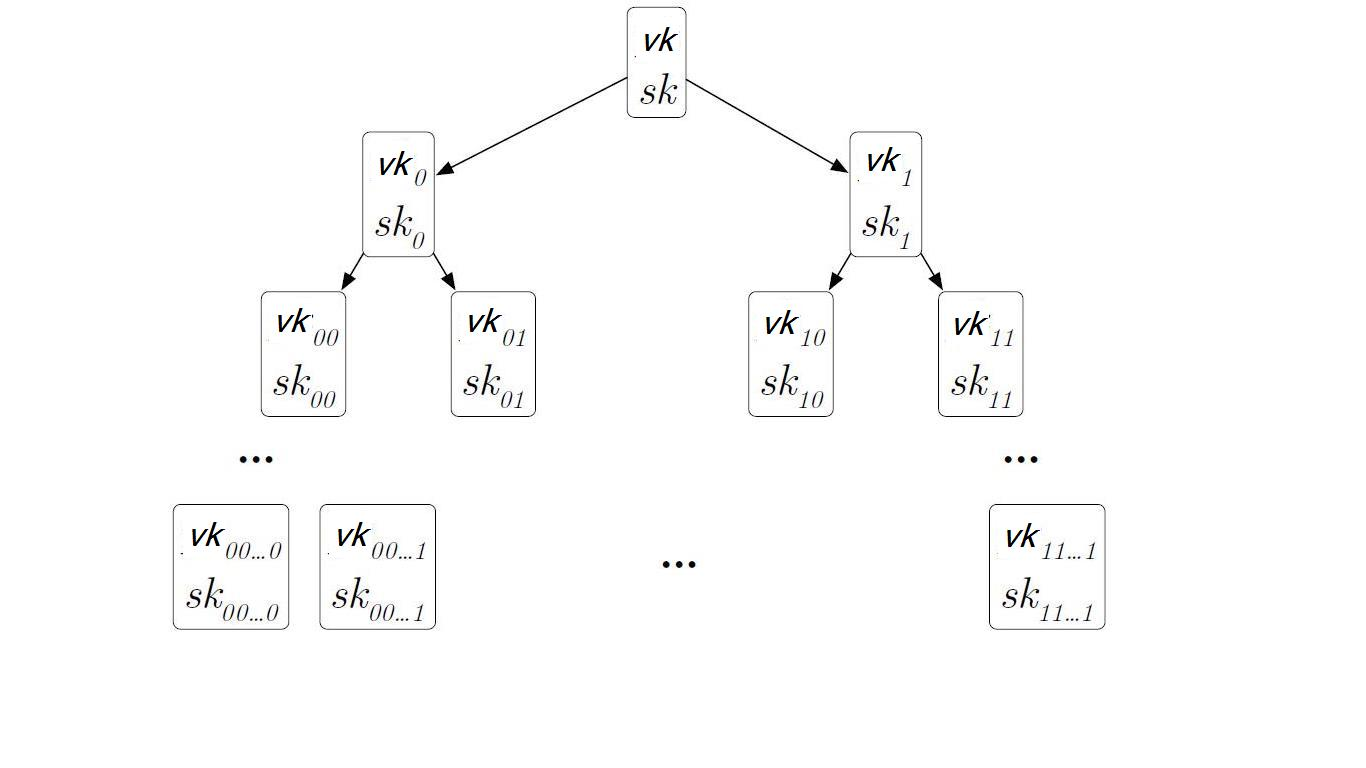
\includegraphics[scale = 0.35]{tree}
\end{center}

At any point of time, the signer maintains a special node which it
calls the \emph{current node}.  To sign a message $m$, if the current
node is at a depth less than $n$ in the tree, the signer generates and
stores $2$ more key-pairs and sets them as the children of the current
node.  It uses the signing key in the current node to sign the message
together with the two new verification keys, and updates the current
node as the left child.  Otherwise, (i.e., if the current node is
already at a depth $n$), the signer uses the current node to sign the
message and updates the current node to be the successor in the
preorder traversal of the tree.

Here the signer need only include a transcript of all the previously
signed messages \emph{down the path from the root to the current
  node}.  In addition, the signer need only keep state containing the
keys along the path to the current node, and their siblings.

Moreover, we can make the scheme entirely \emph{stateless} by viewing
the tree as \emph{implicitly} fully determined by a PRF $f_{k}$.  That
is, in order to generate the key pair at a certain node, the signer
computes $f_{k}$ on a corresponding input, and uses the result as the
random coins for $\ots.\siggen$.  Because $f_{k}$ always returns the
same output on the same input, the signer can consistently regenerate
any desired node as needed.  To sign a message, the signer then just
signs relative to a randomly chosen leaf node.  With high probability,
no leaf is ever used more than once, so (intuitively, at least) the
scheme is secure.  A full proof is rather involved, but not especially
difficult.

\end{document}

%%% Local Variables: 
%%% mode: latex
%%% TeX-master: t
%%% End: 
